\documentclass[11pt]{beamer}
\usepackage[utf8]{inputenc}
\usepackage[T1]{fontenc}
\usepackage{lmodern}
\usepackage{amsmath}
\usepackage{amsfonts}
\usepackage{amssymb}
\usepackage{graphicx}
\usepackage{tikz}
\usepackage{xspace}
\usepackage{hyperref}
\usetheme{Singapore}

\usepackage{environ}
\makeatletter
\newsavebox{\measure@tikzpicture}
\NewEnviron{scaletikzpicturetowidth}[1]{%
	\def\tikz@width{#1}%
	\def\tikzscale{1}\begin{lrbox}{\measure@tikzpicture}%
		\BODY
	\end{lrbox}%
	\pgfmathparse{#1/\wd\measure@tikzpicture}%
	\edef\tikzscale{\pgfmathresult}%
	\BODY
}

\begin{document}
	\author{Quan Gan}
	\title{Recommender Systems and DGL}
	%\subtitle{}
	%\logo{}
	\institute{AWS Shanghai AI Lab}
	%\date{}
	%\subject{}
	%\setbeamercovered{transparent}
	%\setbeamertemplate{navigation symbols}{}
	\begin{frame}[plain]
		\maketitle
	\end{frame}

	\begin{frame}
		\frametitle{Why Recommendation}
		\only<2>{\begin{center}
			\centering
			\Huge \bf We don't want our customers to think (hard).
		\end{center}}
		\only<3-4>{
			\begin{center}
				\centering
				Good relevant recommendations make the customers adhere to us.
				
				\only<3>{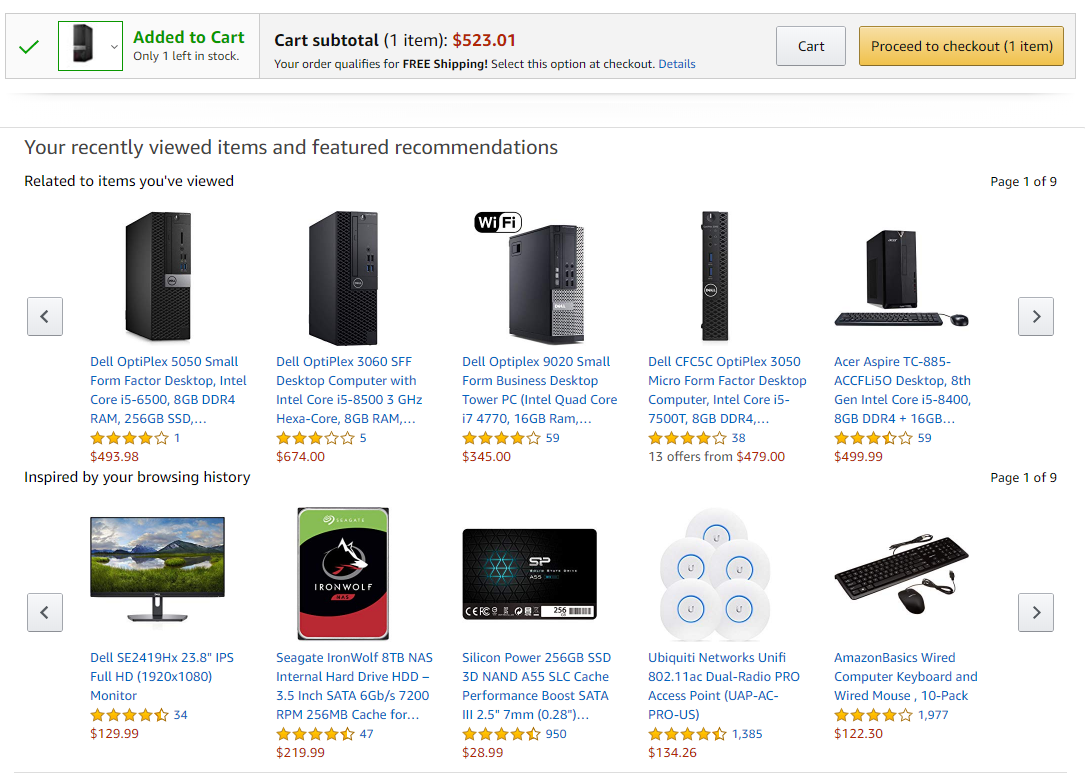
\includegraphics[width=0.8\textwidth]{images/good-recommendation2.png}
				}
				\only<4>{				
\includegraphics[width=0.8\textwidth]{images/good-recommendation.png}}
			\end{center}
		}
	\end{frame}
	
	\begin{frame}
		\frametitle{Recommender System: Problem Statement}
		\begin{center}
			\centering
			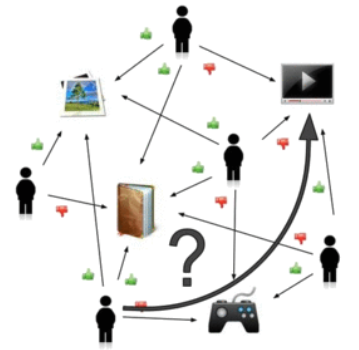
\includegraphics[height=0.7\textheight]{images/cf-stage1.png}
			
			{\tiny Image source: Wikipedia}
		\end{center}
	\end{frame}
	
	\begin{frame}
		\frametitle{Collaborative Filtering}
		\begin{columns}
			\begin{column}{0.3\textwidth}
				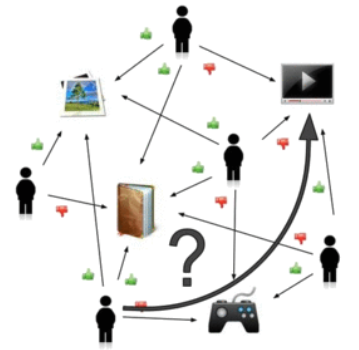
\includegraphics[width=\textwidth]{images/cf-stage1.png}
			\end{column}\pause
			\begin{column}{0.05\textwidth}
				\begin{scaletikzpicturetowidth}{\textwidth}
					\begin{tikzpicture}[scale=\tikzscale]
					\draw [->] (0, 0) -- (0.05, 0);
					\end{tikzpicture}
				\end{scaletikzpicturetowidth}
			\end{column}
			\begin{column}{0.3\textwidth}
				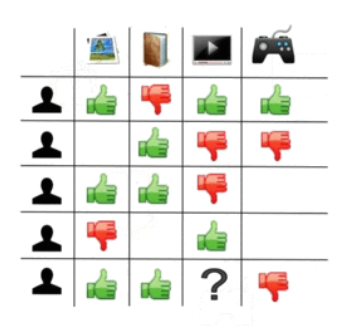
\includegraphics[width=\textwidth]{images/cf-stage2.png}
			\end{column}\pause
			\begin{column}{0.05\textwidth}
				\begin{scaletikzpicturetowidth}{\textwidth}
					\begin{tikzpicture}[scale=\tikzscale]
					\draw [->] (0, 0) -- (0.05, 0);
					\end{tikzpicture}
				\end{scaletikzpicturetowidth}
			\end{column}
			\begin{column}{0.3\textwidth}
				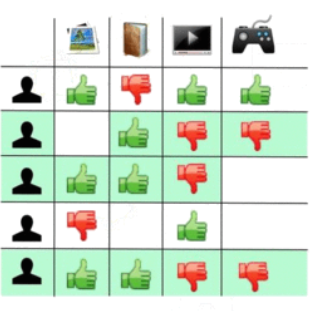
\includegraphics[width=\textwidth]{images/cf-stage3.png}
			\end{column}
		\end{columns}
		\note{Interactions can be inferred by looking at similar users/items.  Users/items are similar if they share some interaction pattern.}
		\begin{center}
			\centering
			{\tiny Image source: Wikipedia}
		\end{center}
	\end{frame}

	\begin{frame}
		\frametitle{Collaborative Filtering: Classical Methods}
		\begin{columns}
			\begin{column}{0.5\textwidth}
				\begin{itemize}
					\item \textbf{User-based}: Infer how a user $i$ would act to an item $j$ by looking at how users that have similar interactions to user $i$ acted to item $j$.
					\begin{itemize}
						\item<2> We have millions of customers.
						\item<3> User profiles change constantly and quickly, requiring frequent rebuilds (which are expensive already).
						\note[item]{Build complexity is $O(U^2I)$}
					\end{itemize}
				\end{itemize}
			\end{column}
			\begin{column}{0.5\textwidth}
				\begin{center}
					\centering
					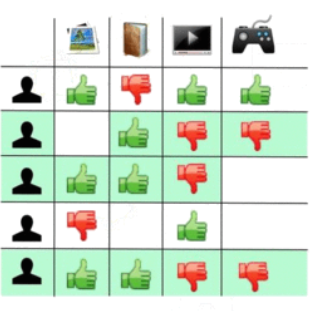
\includegraphics[width=\textwidth]{images/cf-stage3.png}
				\end{center}
			\end{column}
		\end{columns}
	\end{frame}

	\begin{frame}
		\frametitle{Collaborative Filtering: Classical Methods}
		\begin{columns}
			\begin{column}{0.5\textwidth}
				\begin{itemize}
					\item \textbf{\alert<1>{Item}-based}: Infer how a user $i$ would act to an item $j$ by looking at how \alert<1>{items} that have similar interactions to \alert<1>{item $j$} were being acted by \alert<1>{user $i$}.
					\begin{itemize}
						\item Amazon used to have fewer items than users.
						\item<2-> Now we also have millions of items.
						\note[item]{Build complexity is $O(I^2U)$}
					\end{itemize}
				\end{itemize}
			\end{column}
			\begin{column}{0.5\textwidth}
				\begin{center}
					\centering
					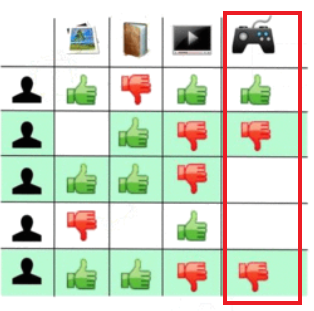
\includegraphics[width=\textwidth]{images/cf-stage3-alter.png}
				\end{center}
			\end{column}
		\end{columns}
	\end{frame}

	\begin{frame}
		\frametitle{Machine Learning Kicks In}
		\begin{columns}
			\begin{column}{0.5\textwidth}
				\begin{center}
					\centering
					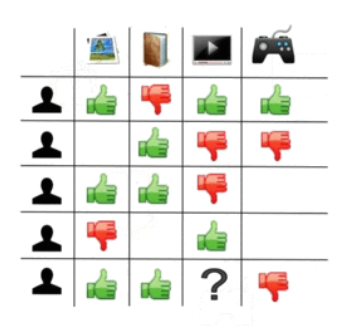
\includegraphics[width=\textwidth]{images/cf-stage2.png}
					
					We were "representing" users and items with the items/users that had interactions with them.
				\end{center}
			\end{column}\pause
			\begin{column}{0.5\textwidth}
				\begin{center}
					\centering
					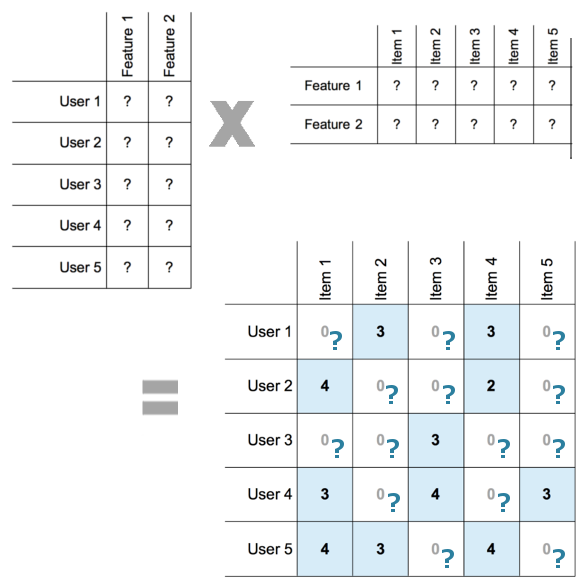
\includegraphics[width=\textwidth]{images/matrix_factorization.png}
					
					{\tiny Source: \href{https://katbailey.github.io/post/matrix-factorization-with-tensorflow/}{\color{blue} Kat Bailey}}
					
					Can we represent users and items as a set of features?
				\end{center}
			\end{column}
		\end{columns}
	\end{frame}

	\begin{frame}
		\frametitle{Content-based recommendation}
		\begin{itemize}
			\item 
		\end{itemize}
	\end{frame}

	\begin{frame}
		\frametitle{Other Meaningful Aspects to Consider}
		\begin{itemize}
			\item \textbf{Cold-start}: What if we have \textit{new} users and items coming in, with few to no historical interactions?
			\item \textbf{Bias correction}: The training dataset usually comes from the result of a \textit{previous recommender system}.  How to mitigate the bias?
			\item \textbf{Diversity}: Always recommending the same items (or even the same kind of item) to a user would make him/her feel \textit{bored}.
		\end{itemize}
	\end{frame}

	\begin{frame}
		\frametitle{Extensions of Matrix Factorization}
		\begin{itemize}
			\item The score function of vanilla MF: $u_i^\top v_j$
			\item RNN To integrate user history, $u_i = f(v_{u, 1}, v_{u, 2}, \cdots, v_{u, n})$
			\item Graph-based models to integrate neighboring items/users (in the next slide).
			\item Can also combine with content-based recommendation (i.e. with user and item features)
		\end{itemize}
	\end{frame}

	\begin{frame}
		\frametitle{Extensions of Matrix Factorization \tiny (with Graph-based Models)}
	\end{frame}

	\begin{frame}
		\begin{center}
			\centering
			\Huge Coding Session
		\end{center}
	\end{frame}
\end{document}